% \begin{landscape}
\begin{figure}[h!]
\begin{center}
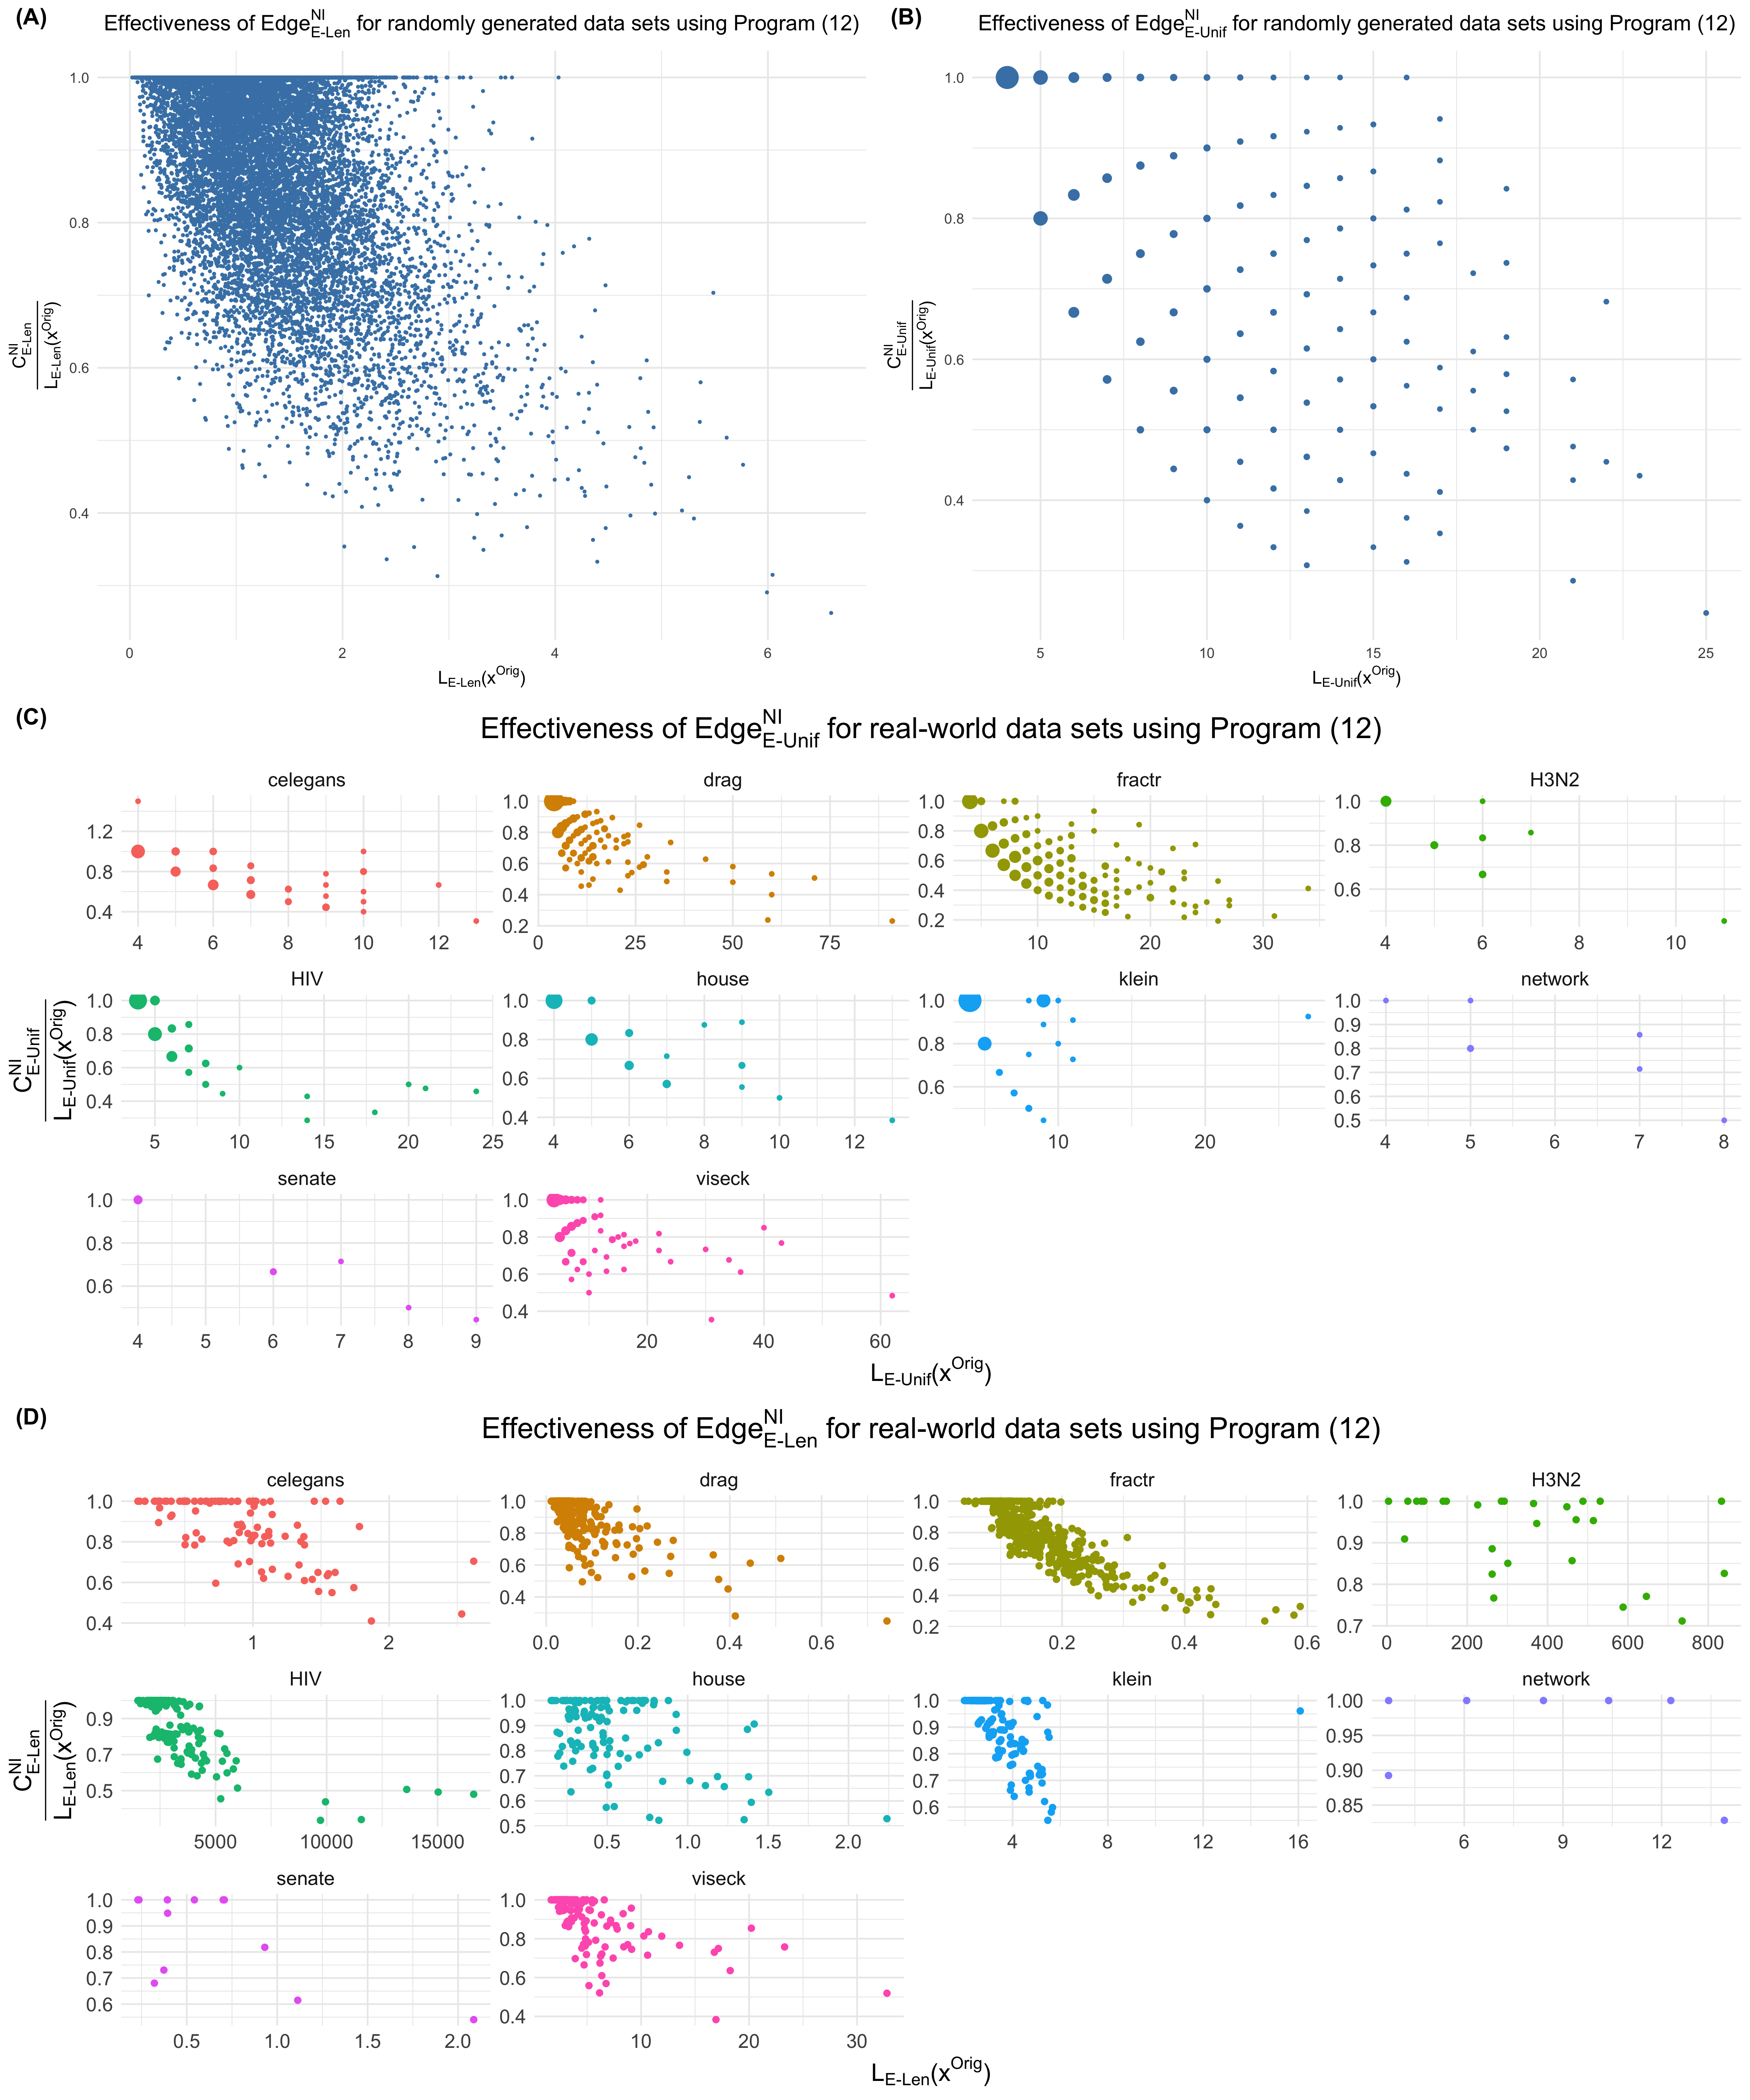
\includegraphics[width=0.95\textwidth]{figures/four_eff_df2.png}% This is a *.eps file
\end{center}
\caption{The effectiveness of length-weighted and uniform-weighted optimization for the randomly generated data sets and real-world data sets in reducing the size of the original cycle representative found by the persistence algorithm. In each subfigure, the horizontal axis is the size of the original representative and the vertical axis is the ratio between the size of the optimal representative and the size of the original representative. The uniform-weighted graphs appear more sparse because reductions in the cost $L_{T\text{-}Unif}(\originalrep)$ can only come in multiples of the reciprocal of the original length. The node size in the uniform-weighed graphs corresponds to the number of overlapping points. %\LL{updated! 0314}
}\label{fig:effectivenessall}
\end{figure}
% \end{landscape}

% \begin{figure}[h!]
% \begin{center}
% 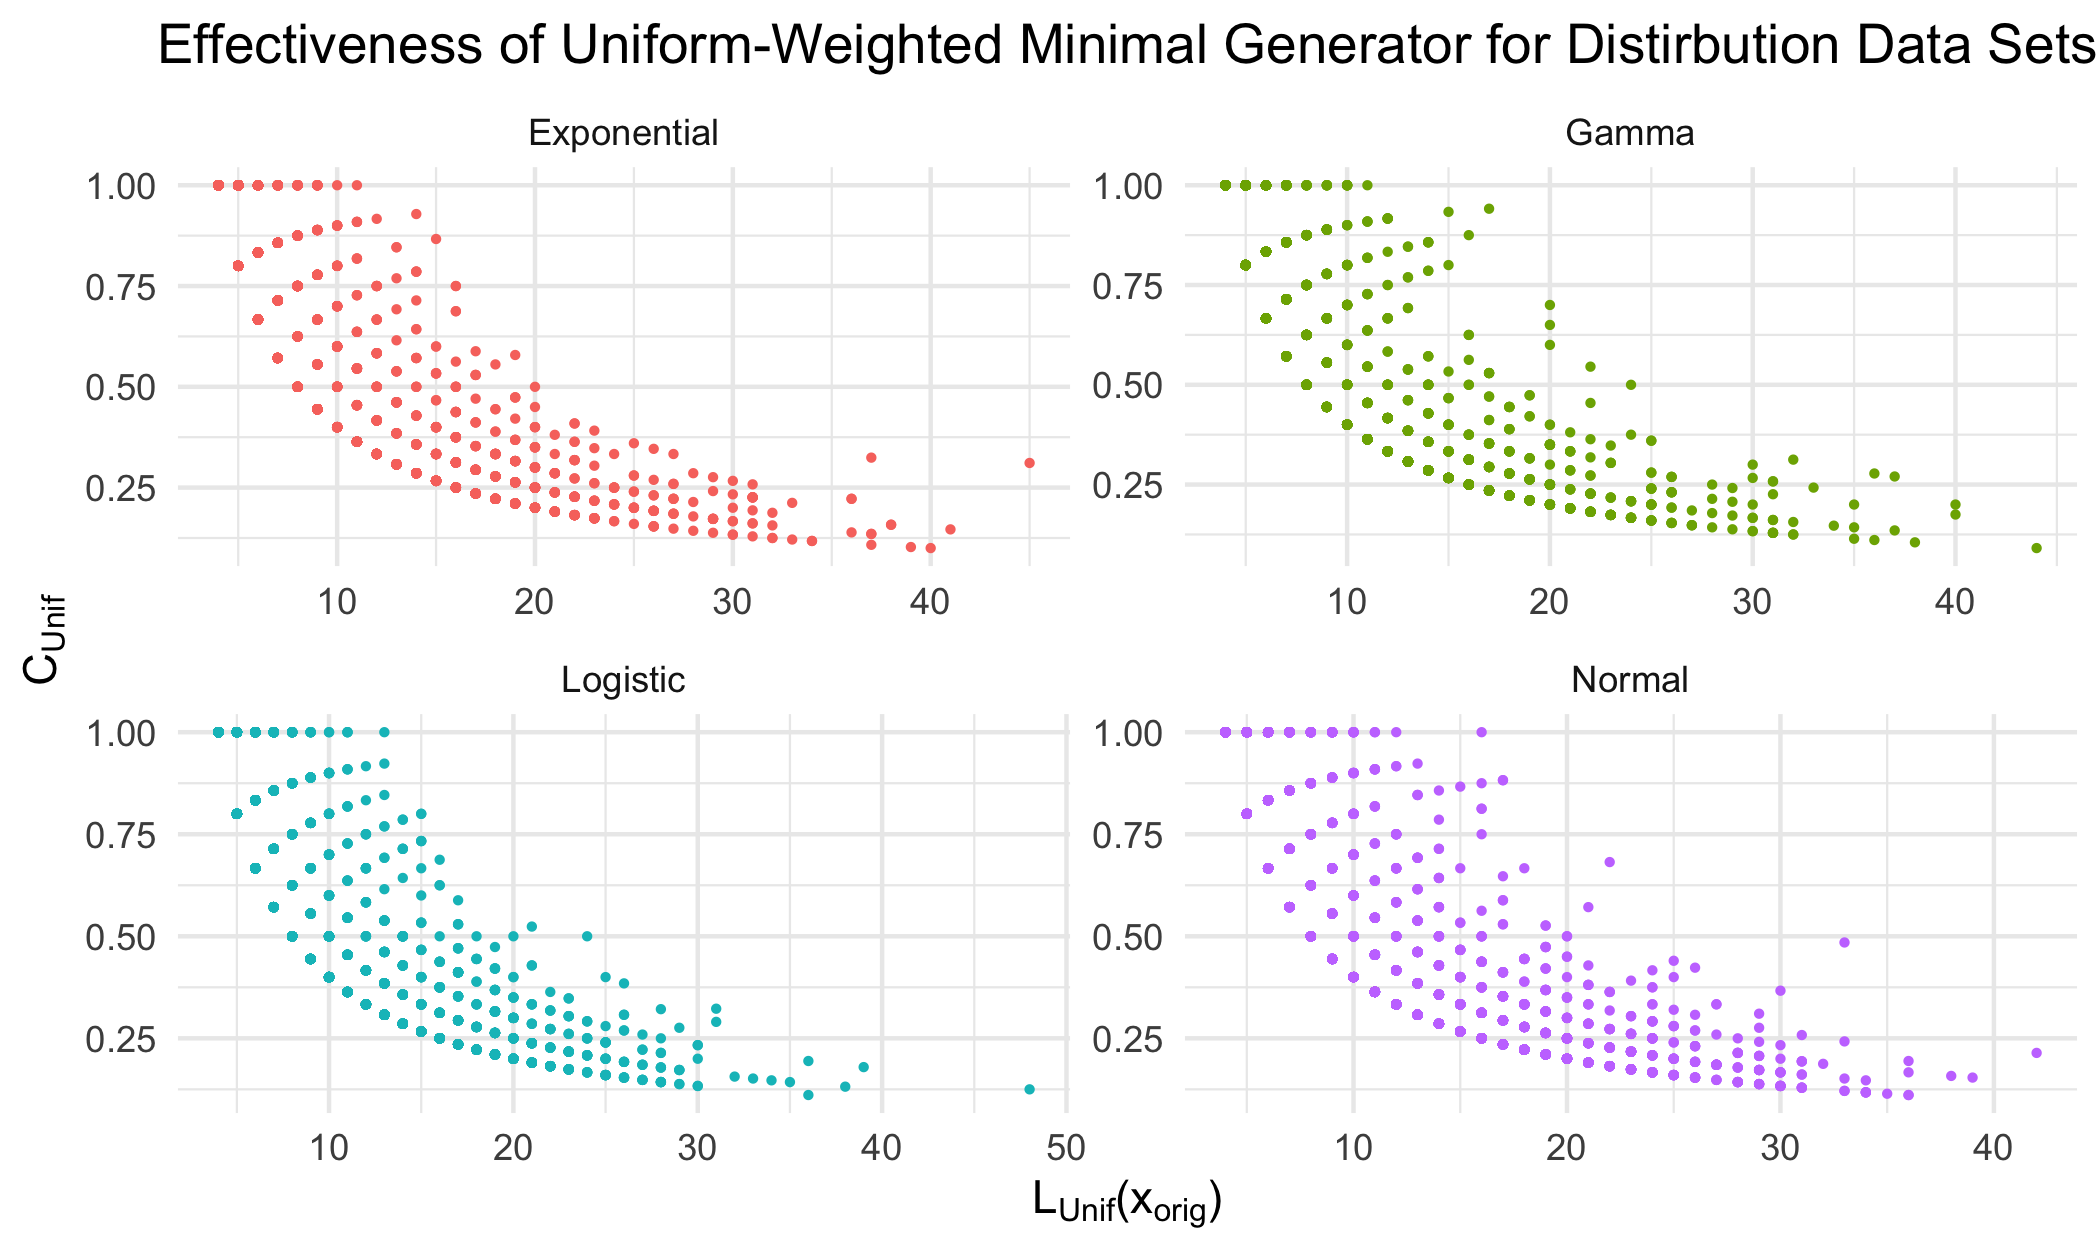
\includegraphics[width=1\textwidth]{figures/edge_eff_dist.png}% This is a *.eps file
% \end{center}
% \caption{Effectiveness of Uniform-Weighted Minimal Generator for Distribution Data Sets}\label{fig:edge_eff_dist}
% \end{figure}

% \begin{figure}[h!]
% \begin{center}
% 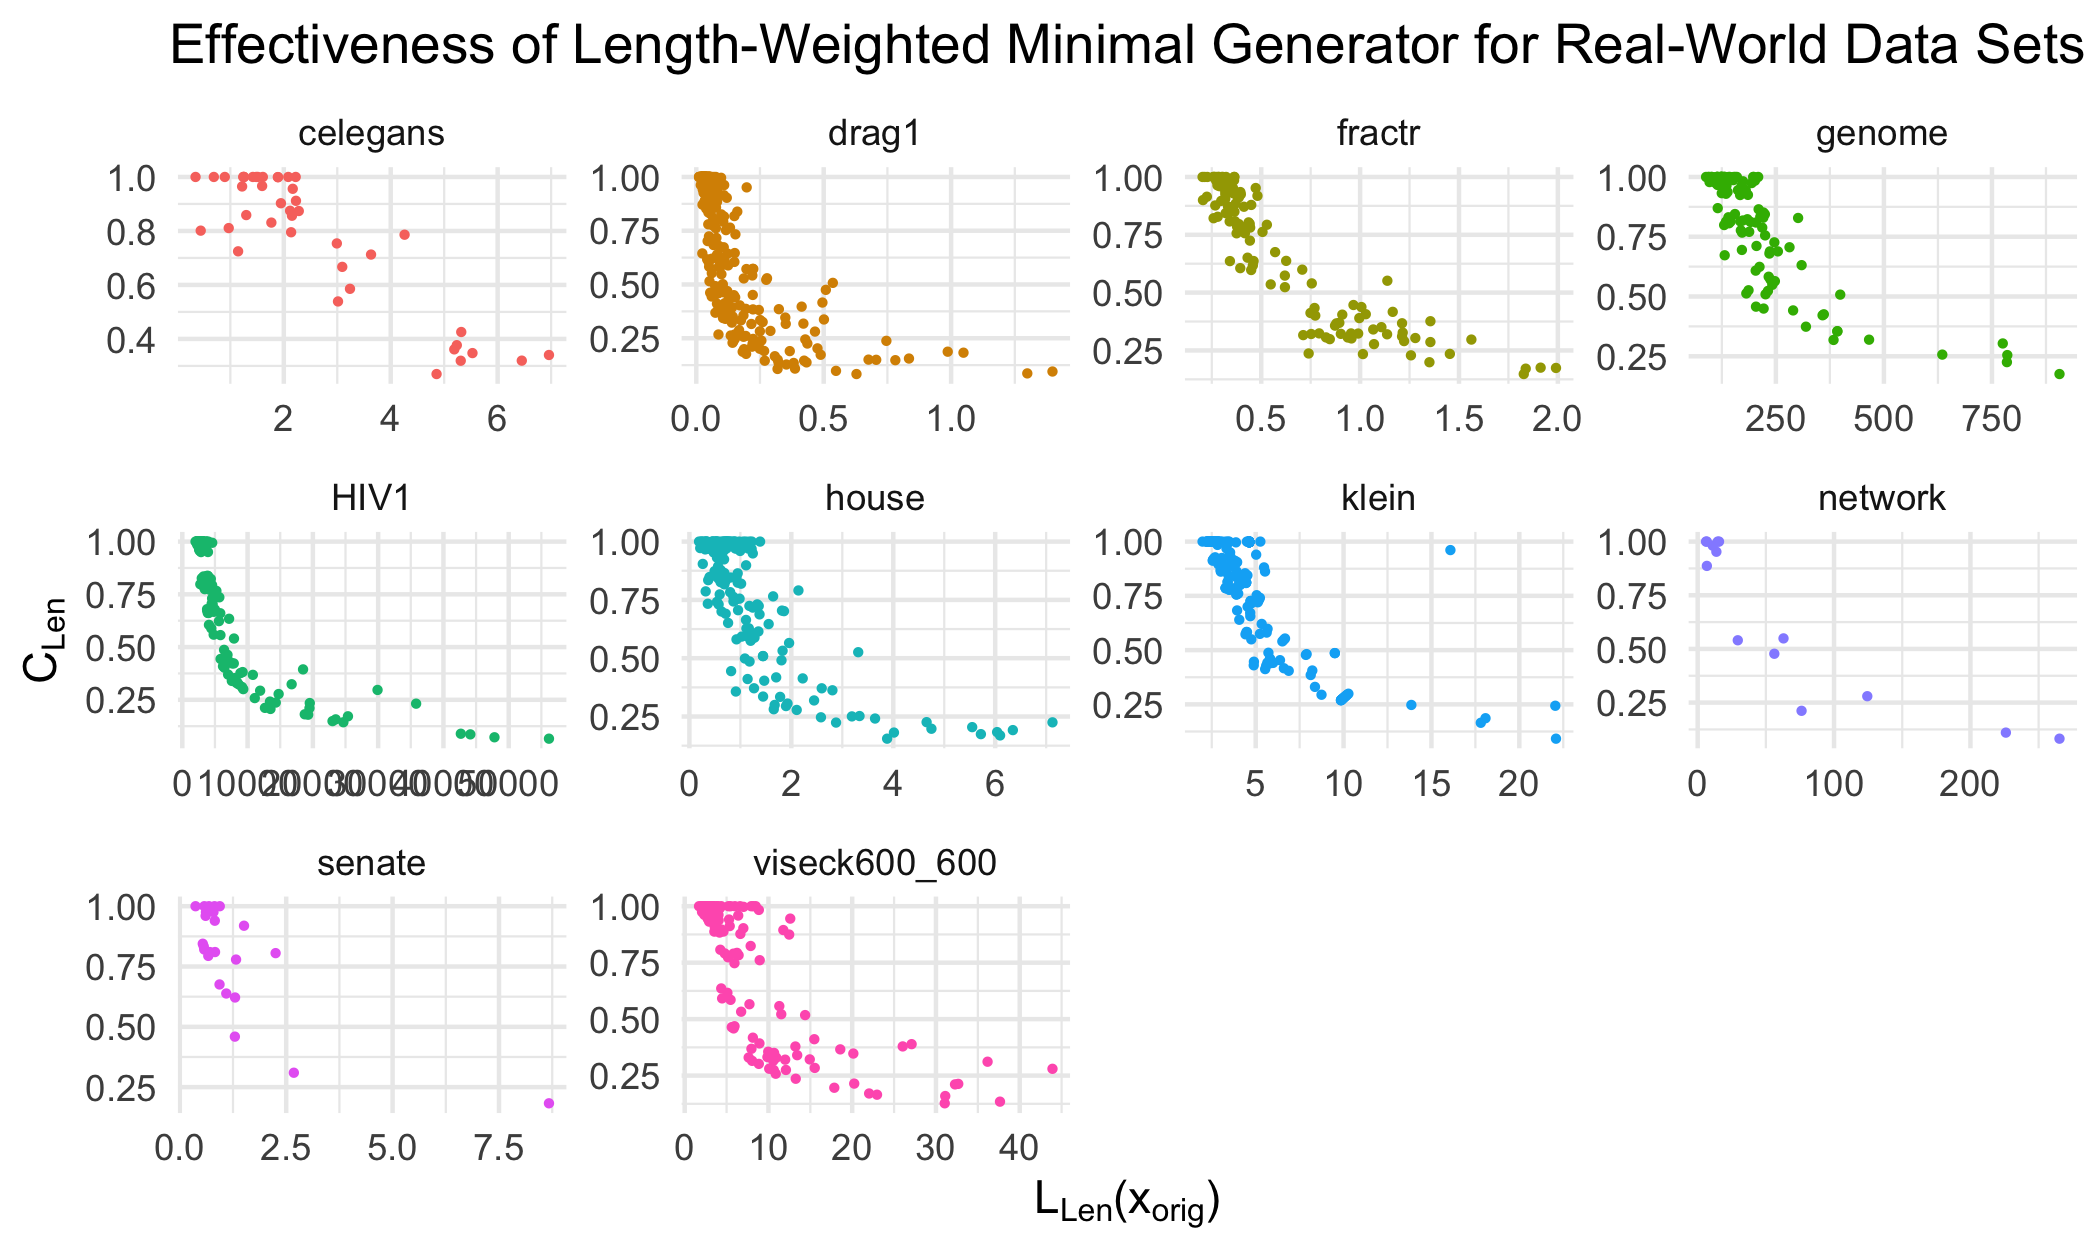
\includegraphics[width=1\textwidth]{figures/length_eff_df.png}% This is a *.eps file
% \end{center}
% \caption{Effectiveness of Length-Weighted Minimal Generator for Real-World Data Sets}\label{fig:length_eff_df}
% \end{figure}
% \begin{figure}[h!]
% \begin{center}
% 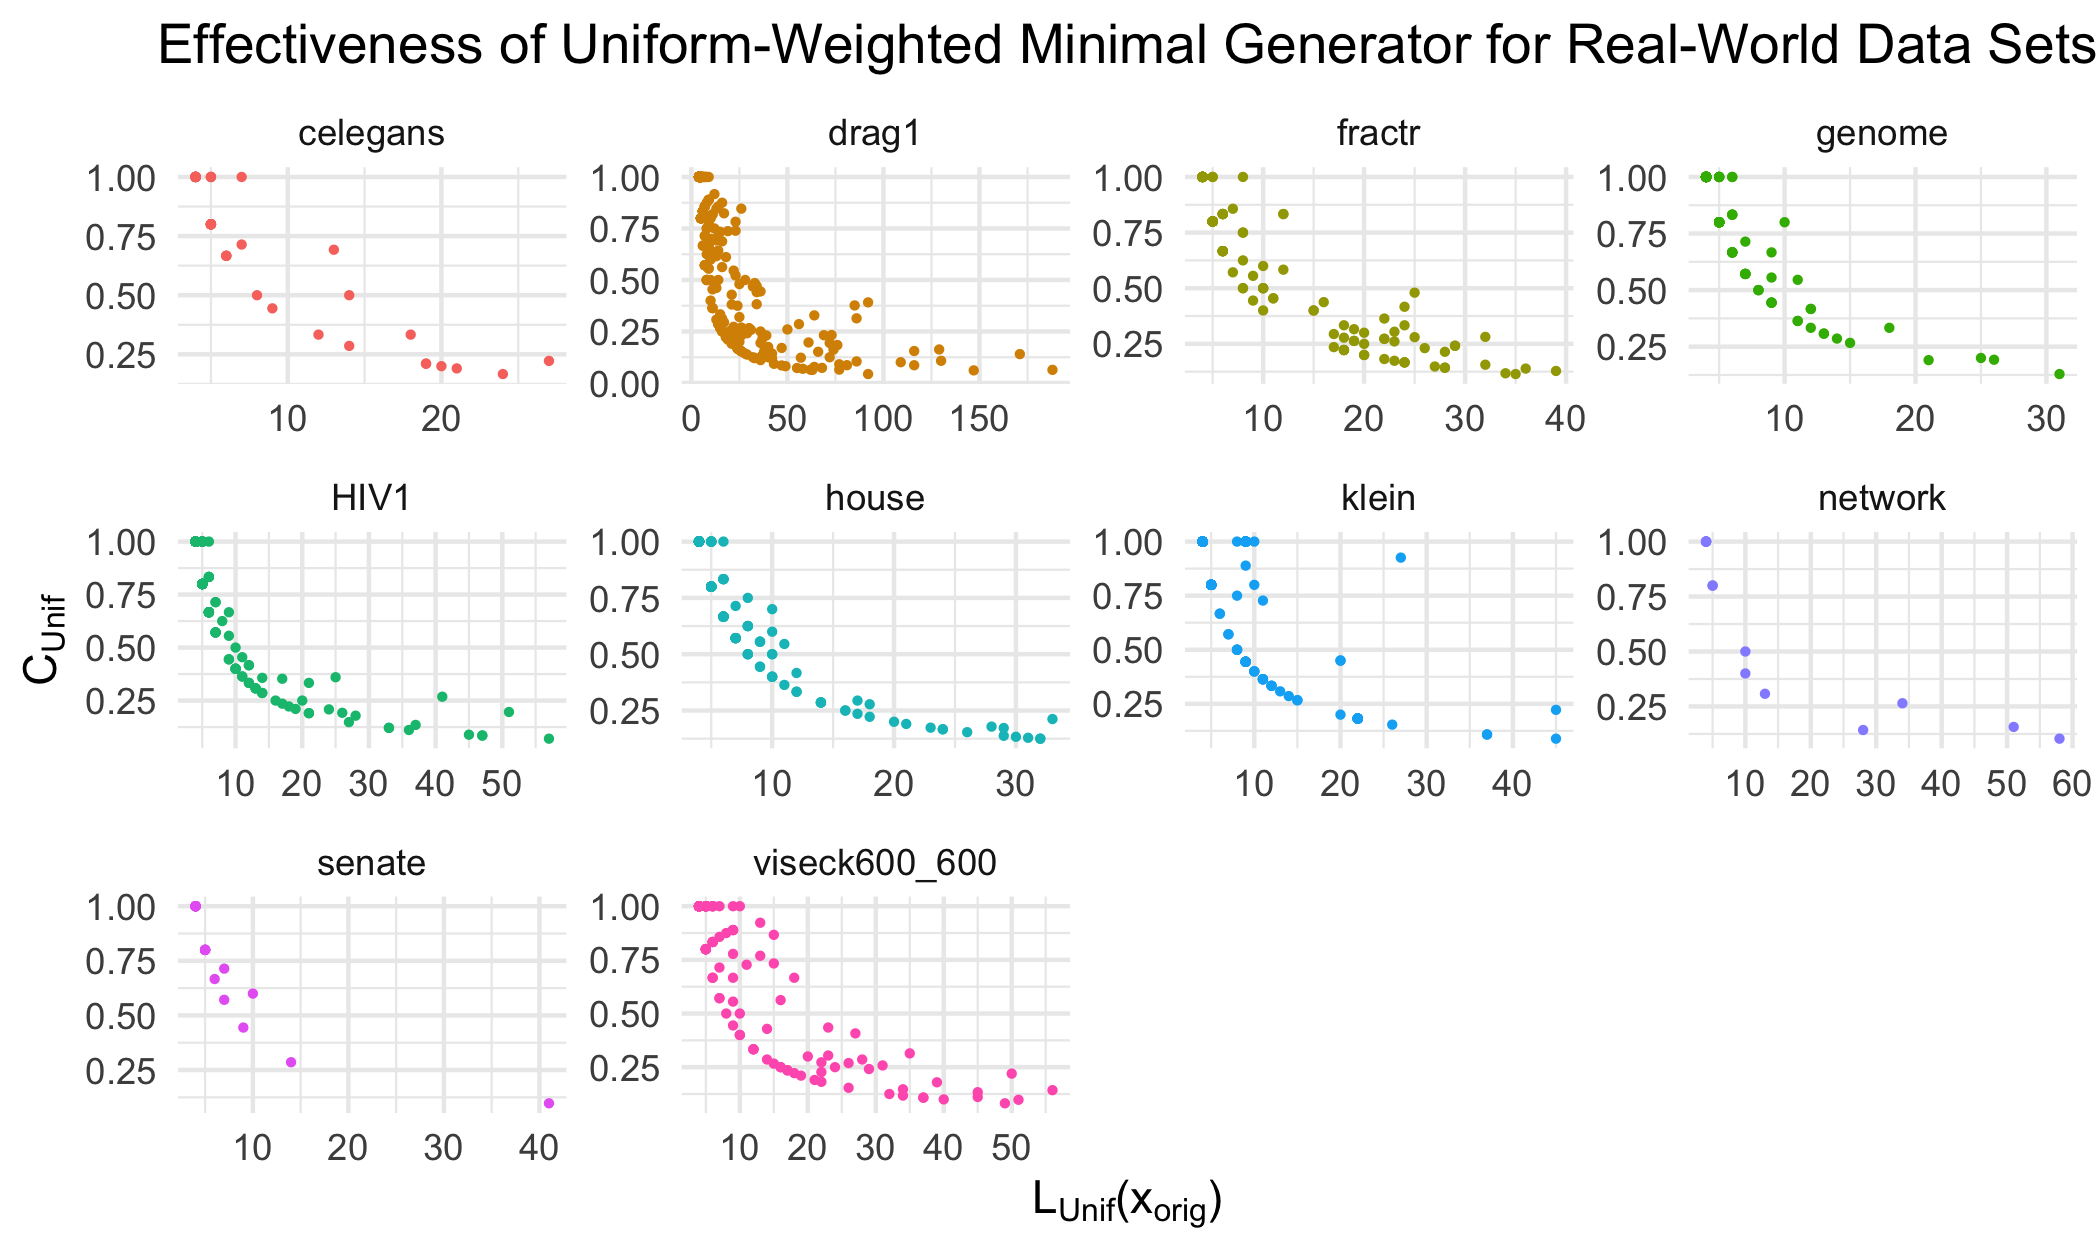
\includegraphics[width=1\textwidth]{figures/edge_eff_df.png}% This is a *.eps file
% \end{center}
% \caption{Effectiveness of Uniform-Weighted Minimal Generator for Real-World Data Sets}\label{fig:edge_eff_df}
% \end{figure}
